\documentclass[11pt]{article}
\usepackage[utf8]{inputenc}
\usepackage[french]{babel}
\usepackage{graphicx}
\usepackage[T1]{fontenc}
\usepackage{lmodern}
\usepackage{amsmath}
\usepackage{amsfonts}
\usepackage{amssymb}
\usepackage{ifthen}
\usepackage{multicol}
\usepackage{fancyhdr}
\newcommand{\marge}{18mm}
\usepackage[left=\marge,right=\marge,top=\marge,bottom=\marge]{geometry}
\pagestyle{fancy}
\setlength{\headheight}{14pt}
%\chead{\ifthenelse{\thepage=1}{
%\textbf{Nom :}
%\makebox[12em]{\dotfill}
%\hspace{2em}
%\textbf{Pr\'enom :}
% \makebox[12em]{\dotfill}}{}}
\rfoot{\ifthenelse{\thepage=1}{\textit{(tournez la page s.v.p)}}{}}
\renewcommand{\headrulewidth}{0pt}
\linespread{1.3}
\setlength{\columnseprule}{0.2pt}
 
% Commandes sp\'ecifiques pour les QCM
\newboolean{correction}
% true pour afficher la correction
% false pour la masquer
\setboolean{correction}{false}
\newcounter{QNumber}
\newcommand{\Question}[2][ ]{
 \stepcounter{QNumber}
  \noindent\textbf{Question \theQNumber} --
  #2~#1}
\newenvironment{Reponse}{
 \begin{list}{$\square$}{\leftmargin=4em}}{
 \end{list}\vspace{1em}}
\newcommand{\Vrai}{
 \item[\ifthenelse{\boolean{correction}}{$\blacksquare$}{$\square$}]}
\newcommand{\Faux}{\item[$\square$]}
\newcommand{\comment}[1]{}
 
\def\N{\mathbb N}
\def\R{\mathbb R}
\def\Q{\mathbb Q}
\def\Z{\mathbb Z}
\begin{document}
  \begin{center}
    \bfseries\LARGE
    \textit{INFO I31, examen 2012}\large
  \end{center}
  \sffamily
  \begin{itshape}
  \begin{multicols}{2}
 
\Question{Algorithme d'Euclide \'etendu.}
Soient $a\in \N, b\in \N$ avec $0 \le a \le b$. La fonction $BZ: (a,b)\rightarrow (x,y,g)$
est telle que $g$ est le PGCD de $a$ et $b$, et $x, y$ sont deux entiers relatifs (de $\Z$)
tels que $ax+by=g$. Compl\'etez la d\'efinition suivante~:
$BZ(0, b)=(0,1,b)$;  et
$BZ(a>0, b)= ( ?, ?, g)$ o\`u
$q$ est le quotient de $b$ par $a$ (division euclidienne),
$r=b \mod a$,
et $(x',y',g)=BZ(r, a)$.

\Question{Pour $(a, b)$ donn\'es, les $(x, y)$ de Bezout ne sont pas uniques.
D\'ecrivez tous les $(x_k, y_k)$ solutions pour $(a, b)$ quelconque et un couple
$(X,Y)$ solution.}

\Question{D\'eroulez la m\'ethode d'Euclide \'etendue 
pour $(a, b)=(55, 89)$, dans un tableau
avec les colonnes $a, b, q=\lfloor \frac{b}{a}\rfloor, r=b \mod a, x, y, g$ (\`a chaque ligne,
$ax+by=g$ doit \^etre vraie)}
 
\Question{Citez un premier probl\`eme ind\'ecidable (insoluble).}

\Question{Citez en un second.}

\Question{Citez un  premier probl\`eme difficile sur les graphes ("difficile": dont on ne connait pas de m\'ethode en temps polynomial dans le pire des cas)}

\Question{Citez en un second.}

\Question{Pour quelle valeur de $k>1$ est il toujours 
facile de d\'ecider si un graphe non orient\'e donn\'e  est
coloriable en $k$ couleurs, et facile de trouver un tel coloriage s'il en existe un~?} 

\Question{Donnez les formules r\'ecursives pour le calcul {\bf rapide} de $a^k$, o\`u
$a$ est une matrice carr\'ee, et $k\in \N$}

\Question{Donnez la formule matricielle permettant de calculer $F_n$, o\`u $F_n$ est
le $n$ i\`eme nombre de Fibonacci~: $F_0=0, F_1=1, F_n=F_{n-1}+F_{n-2}$ quand $n>1$}

\Question{Le probl\`eme SAT consiste \`a trouver les valeurs des inconnues bool\'eennes $x=(x_1, x_2,\ldots x_n)$
(vrai ou faux) qui rendent vraie une formule donn\'ee, telle que: $(x_1 \vee x_2 \vee \neg x_3)$ et $x_4 \vee x_5  \vee \neg x_7)$ et $\ldots$. Aucune m\'ethode en temps polynomial en
$n$ n'est connue. Donnez le nombre de valeurs possibles pour
$x$ (qui satisfasse ou non la formule) pour $n$ quelconque}

\Question{Pour $n=30000$, convertissez le nombre pr\'ec\'edent en puissance de 10, en utilisant $2^{10}\approx 10^3$.}

\Question{$2^{10}\approx 10^3 \Rightarrow \frac{\log 2}{\log 10}\approx ??$}


\begin{center}
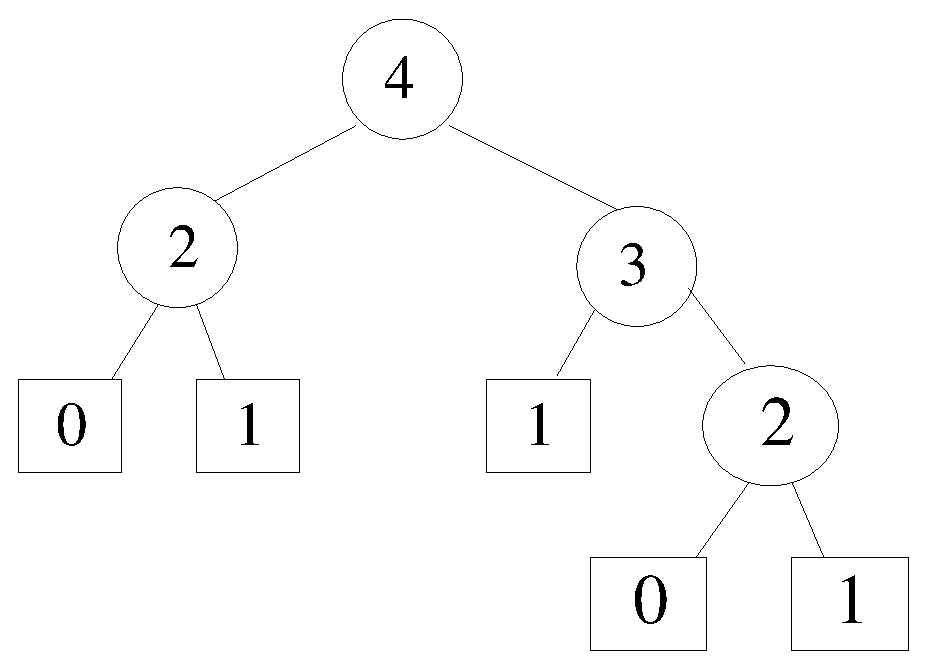
\includegraphics[width=0.5\linewidth]{arbreFibonacci.eps}
\end{center}

\Question{L'arbre de Fibonacci $T_4$ est dessin\'e ci-dessus. $T_0$ est une feuille portant l'\'etiquette 0,
$T_1$ est une feuille portant  l'\'etiquette 1; pour $n>1$, 
$T_n$ est un noeud binaire, dont le fils gauche est $T_{n-2}$ et 
dont le fils droit est $T_{n-1}$. 
%Donnez une formule r\'ecursive pour 
%le nombre d'\'el\'ements (feuilles ou sommets), not\'e $|T_n|$,  de $T_n$, pour $n>1$}
%\Question
Remplissez un tableau avec les lignes $n$,
$I_n$, $U_n$, $Z_n$ et les colonnes $n=0, 1\ldots 8$~:   
$U_n$ est le nombre de feuilles \'etiquet\'ees 1 de $T_n$,
$Z_n$ le nombre de feuilles \'etiquet\'ees 0 de $T_n$, 
$I_n$ le nombre de noeuds int\'erieurs (non feuilles)  de $T_n$. Donnez des formules r\'ecursives d\'efinissant  $U_n, Z_n, I_n$.
Quelle relation  remarquez vous entre $U_{n+1}$ et $I_n$? Aucune preuve n'est demand\'ee.}

%	\comment{
%	$$
%	\begin{array}{|c|c|c|c|c|c|c|c|c|c|c|}
%	\hline
%	n & 0 & 1 & 2 & 3 & 4 & 5 & 6 & 7 & 8 & 9 \\
%	\hline
%	I_n & & & & & & & & & &  \\
%	\hline
%	U_n & & & & & & & & & &  \\
%	\hline
%	Z_n & & & & & & & & & &  \\
%	\hline
%	\end{array}
%	$$
%	}


\Question{Le temps d'ex\'ecution d'un algorithme  est
$T(n)$ pour une donn\'ee de taille $n$, o\`u $T(1)=1$ et $T(n)=3 T(n/2)+n$.
{\bf Prouver par r\'ecurrence} que $T(2^k) = 3^{k+1}\alpha + 2^{k+1}\beta$ pour des
constantes $\alpha, \beta$ que vous d\'evinerez. Pour vous aider, remplissez d'abord  le
tableau: $n=2^k, k, T(n), 3^{k+1}, 2^{k+1}$ pour $k$ de 0 \`a 4. Inutile d'\'ecrire ce tableau sur votre copie}


\Question{Prouvez que $3^{\log_2 n}$ est en $O(n ^{log_3 2})$ (Remarque: $\log_3 2\approx 1.5849625$)}





\comment{
\Question{Pour le calcul de l'arbre couvrant minimum d'un graphe connexe, 
un \'etudiant propose l'algorithme suivant: si le graphe est un arbre, alors ins\'erer cet arbre dans l'arbre couvrant minimum;
sinon d\'ecomposer le graphe $G$ en 2 graphes de taille \`a peu pr\`es moiti\'e, $G_1$, et $G_2$, tous deux connexes; calculer
l'arbre couvrant minimum de $G_1$; calculer l'arbre couvrant minimum de $G_2$; joindre ces deux arbres par l'ar\^ete de co\^ut
 minimum entre $G_1$ et $G_2$ (cette ar\^ete a un sommet dans $G_1$ et un sommet dans $G_2$).
Que pensez-vous de cet algorithme} 
\begin{Reponse}
\Faux il est correct
\Faux il est difficile de partitionner un graphe connexe en deux sous graphes connexes ayant (\`a peu pr\`es) deux fois moins de sommets; c'est pourquoi cet algorithme n'est pas utilis\'e
\Vrai il est incorrect, et voici un contre exemple simple (au plus 4 sommets!) :
\end{Reponse}
}




\Question{Arthur conjecture que si, dans un graphe non orient\'e, tous les sommets distincts soit sont voisins, 
soit ont un voisin en commun, alors il existe au moins un sommet qui est voisin de tous les autres.  Que pensez vous de cette conjecture}
\begin{Reponse}
\Faux elle est vraie
\Vrai elle est fausse et vous en dessinez un contre exemple simple 
\end{Reponse}

Soient trois ensembles finis donn\'es $E, F, G$.
$A$ et $B$ sont des matrices, telles que $A_{ef}$ est le co\^ut de l'arc de $e\in E$ \`a $f\in F$, et $B_{fg}$ est le co\^ut de l'arc de $f\in F$ \`a $g\in G$
(s'il n'y a pas d'arc, on utilise $\infty$).
Le co\^ut minimum $C_{eg}$ de $e\in E$ \`a $g\in G$ est $\min_{f\in F} A_{ef}+B_{fg}$.
Les questions suivantes g\'en\'eralisent ces notions.

\Question{$A_{ef}$ est la probabilit\'e de mourir en utilisant l'arc $e\rightarrow f$;
$B_{fg}$ est la probabilit\'e de mourir en utilisant l'arc $f\rightarrow g$.
Quelle est la probabilit\'e de mourir, en utilisant le chemin le moins risqu\'e pour aller de $e\in E$ \`a $g\in G$~? (on demande une formule, pas un algorithme!)}
 
\Question{
Ici, les matrices $A$ et $B$ sont des matrices donnant
la probabilit\'e du passage d'un sommet \`a un autre dans un graphe sous jacent. 
Ces matrices sont appel\'ees matrices de Markov, ou matrices stochastiques. Par exemple, 
$E, F, G$ sont respectivement des noms (ou groupes nominaux: "le chat"), des verbes, des adjectifs.
$A_{ef}$ est la probabilit\'e pour que le mot $e\in E$, qui vient d'\^etre prononc\'e,
soit suivi du mot $f\in F$. De m\^eme $B_{fg}$ est la probabilit\'e pour que le mot
$f\in F$, qui vient d'\^etre prononc\'e, soit suivi du mot $g\in G$.
Or une probabilit\'e v\'erifie certaines conditions (par exemple, appartenir \`a $[0, 1]$).
Quelle est la condition suppl\'ementaire sur, disons, la matrice  $A$, qui n'\'etait pas 
indispensable pour  la question pr\'ec\'edente~?}

\Question{(Suite)
Quelle est la probabilit\'e de la phrase sujet-verbe-adjectif 
la plus probable qui commence par $e$ et se termine par $g$~? ou~: quelle
est la probabilit\'e du chemin le plus probable qui commence en $e$ et se termine en $g$~?} 


\Question{
(Suite) Quelle est la probabilit\'e qu'une "phrase" (un chemin)
qui commence en $e$ ($e\in E$) se termine en $g$ ($g\in G$)~?}



\comment{
\Question{$E$ est un ensemble de mots anglais, $F$ un ensemble de mots
fran\c{c}ais,  $G$ est un ensemble de mots allemands. 
$A_{ef}$ est la probabilit\'e pour qu'un logiciel de traduction automatique
traduise le mot anglais $e\in E$ par le mot fran\c{c}ais $f\in F$.
De m\^eme $B_{fg}$ est la probabilit\'e pour qu'un logiciel de traduction automatique traduise le mot   fran\c{c}ais $f\in F$ par le mot allemand $g\in G$.
Quelle est la probabilit\'e
pour que l'enchainement des deux logiciels traduise $e\in E$ en $g\in G$~?}
}



\Question{Vous devez additionner $n$ nombres flottants positifs donn\'es, par exemple $n=10^6$, et les $n$ nombres sont dans un tableau $T[]$. 
Donnez un exemple simple o\`u il y a une grande impr\'ecision. }

\Question{Proposez un algorithme, ou son principe, pour  limiter l'impr\'ecision num\'erique.}

{
\Question{Logique. $P_1$: tous les chats ne sont pas verts. $Q_1$: aucun chat n'est vert.
$P_2$: tous les corbeaux ne sont pas blancs. $Q_2$: aucun corbeau n'est blanc.
Etc.
Plus g\'en\'eralement, $P$: tous ces $A$ ne sont pas $B$, et $Q$: aucun de ces $A$ n'est $B$.
A-t-on}
\begin{Reponse}
\Faux $P \Leftrightarrow Q$ : $P$ et $Q$ sont \'equivalents
\Faux $P \Rightarrow Q$ : $P$ implique $Q$.
\Faux $Q \Rightarrow P$ : $Q$ implique $P$.
\Faux \c{C}a d\'epend des cas
\end{Reponse}

\Question{Logique. Voici une preuve par r\'ecurrence que tous les corbeaux sont de la m\^eme couleur.
C'est vrai pour 0 corbeau et pour 1 corbeau. Prouvons  que si c'est vrai pour
$n$ corbeaux, alors c'est vrai pour $n+1$ corbeaux. Les $n+1$ corbeaux
sont $C_1, C_2, \ldots C_n, C_{n+1}$. Les $n$ premiers  corbeaux: $P=( C_1, \ldots C_n)$ sont de la m\^eme
couleur (par hypoth\`ese de r\'ecurrence); les  $n$ derniers corbeaux: $D=(C_2, \ldots C_n, C_{n+1})$ sont de la m\^eme
couleur (par hypoth\`ese de r\'ecurrence); mais ces deux ensembles ont en commun $n-1$ corbeaux $I=(C_2, \ldots C_n)$, 
qui sont de la m\^eme couleur; donc les corbeaux  
de $I$ sont de la m\^eme couleur que ceux de $P$ (car $I\subset P$), et ceux de $D$ (car $I\subset D$).
Que pensez vous de ce raisonnement par r\'ecurrence~?}
\begin{Reponse}
\Faux il est correct (d'ailleurs tous les corbeaux sont noirs);
\Vrai il est incorrect. O\`u est  la faille~?
\end{Reponse}
}


\end{multicols}
\end{itshape}
\end{document}
{
\Question{Prolongez de fa\c{c}on logique la suite de Fibonacci aux nombres n\'egatifs}
$$\begin{array}{|c|cccccccccccc|}
\hline
i & -6 & -5 & -4 & -3 & -2 & -1 & 0 & 1 & 2 & 3 & 4 & 5  \\
\hline
F_i & & & & & & & 0 & 1 & 1 & 2 & 3 & 5  \\
\hline
\end{array}
$$


\Question{Vous constatez que, pour $n\in \N$,  $F_{-2n}$ est \'egal \`a}

~\\

\Question{Vous constatez que, pour $n\in \N$,  $F_{-2n-1}$ est \'egal \`a}

~\\
 

\Question{ Soient $\phi=\frac{1}{2}(1+\sqrt{5})\approx 1.618$ et $\phi'=\frac{1}{2}(1-\sqrt{5})\approx -0.618$~; ce sont les deux racines de $x^2-x-1=0$. 
D\'efinissons $f(n)=\frac{1}{\sqrt{5}}(\phi^n - \phi'^n)$.
Donnez la valeur de $f(0), f(1), f(2), f(3)$} 

\Question{Par r\'ecurrence, prouvez que $F_n=f(n)$}

~\\
~\\
~\\
~\\
~\\
}
{
\Question{Une matrice de Vandermonde a la structure suivante~:
$$M= \left( \begin{array}{ccccc}
1 & 1 & 1 & \ldots & 1 \\
1 & w & w^2 & \ldots & w^{n-1} \\
1 & w^2 & w^4 & \ldots &  w^{2(n-1)} \\
\ldots & \ldots & \ldots & \ldots \\
1 & w^{n-1} &  w^{2n-2} &  \ldots & w^{(n-1)^2} \\
\end{array} \right)
$$ o\`u $n$ est une puissance de 2.
Si de plus $w$ est une racine $n$ i\`eme de l'unit\'e, alors le produit avec un vecteur colonne quelconque de taille $n$}
\begin{Reponse}
\Vrai peut se faire en $O(n \log n)$ (avec l'algorithme de la transform\'ee rapide de Fourier) 
\Vrai ne  peut pas se faire en moins que  $O(n)$
\Faux ne peut pas se faire en moins que $O(n^2)$
\end{Reponse}

\Question{Pour $n=8$ (donc $w^8=1$), \'ecrire la ligne de la matrice de Vandermonde commen\c{c}ant par $1$ puis  $w^3$, en simplifiant
(c'est \`a dire en \'eliminant les puissances plus grandes que 7)}

~\\
~\\
~\\
~\\

\Question{Idem, pour $n=8$, \'ecrire la ligne de la matrice de Vandermonde commen\c{c}ant par $1$ puis  $w^6$}

~\\
~\\
~\\
~\\
}
{
\Question{
Un \'etudiant programme le tri rapide ("quicksort") d'une liste $L$ ainsi~: si $L$  contient moins de 2 \'el\'ements, alors elle est d\'ej\`a tri\'ee. Sinon, l'\'etudiant choisit un \'el\'ement $p$  dans $L$. Il partitionne $L$  
en 3 sous listes, la liste $L_1$ des \'el\'ements dans $L$ inf\'erieurs \`a $p$, la liste $L_2$ des \'el\'ements dans $L$
\'egaux \`a $p$,  
la liste $L_3$  des \'el\'ements dans $L$ sup\'erieurs \`a $p$. Il trie r\'ecursivement les 3 listes, puis concat\`ene les r\'esultats. 
Qu'en pensez-vous}
\begin{Reponse}
\Faux la m\'ethode est correcte mais la complexit\'e est modifi\'ee
\Faux la m\'ethode est correcte et la complexit\'e est inchang\'ee
\Vrai la m\'ethode est incorrecte ; elle boucle quand  $L$ contient deux (ou davantage) \'el\'ements \'egaux \`a $p$.
\Faux la m\'ethode est incorrecte car $L_2$ n'est jamais vide, puisqu'elle contient $p$.
\end{Reponse}
}
{
\Question{Dans le probl\`eme de la somme, un ensemble $E$ de $n$ entiers positifs $e_1 \ge e_2 \ge \ldots \ge e_n$ est donn\'e, ainsi
qu'un entier $0<S < \sum_1^n e_i$. Il faut trouver le sous ensemble $X$ de $E$ dont la somme des \'el\'ements
est maximum, mais inf\'erieure ou \'egale \`a $S$.  Pour tout ensemble $K$, on note $\sigma(K)$ la somme des \'el\'ements de $K$.
L'algorithme glouton calcule $X_0=\emptyset$ (donc $s(X_0)=0$);  puis, 
pour $i$ de 1 \`a $n$, il calcule $X_i= X_{i-1} \cup \{e_i\}$ si $e_i + \sigma(X_{i-1}) \le S$, et
$X_i= X_{i-1}$ sinon. Avec $E=100,25,20,10,1,1,1$ et $S=40$, donnez les valeurs de $X_0, X_1, \ldots X_7$, et les $\sigma(X_i)$ correspondants}

~\\
~\\
~\\
~\\
~\\
~\\
~\\

\Question{
Cet algorithme donne-t-il un sous ensemble $X_n$}
\begin{Reponse} 
\Vrai toujours correct ($s(X_n)\le S$), mais pas forc\'ement optimal : donnez un exemple simple ($n<5$) o\`u $X_n$ n'est pas optimal\\
~
\Faux toujours correct, et toujours optimal
\Faux pas toujours correct, mais optimal :  donnez un exemple simple ($n<5$) \\
~ 
\Faux souvent correct, et souvent optimal
\Faux ni correct ni optimal : donnez un exemple simple ($n<5$) \\
~
\Faux toutes les r\'eponses pr\'ec\'edentes sont fausses 
\end{Reponse}

}
